\section{Polynomial Hierarchy, Alternating TMs}

\begin{figure}
\centering
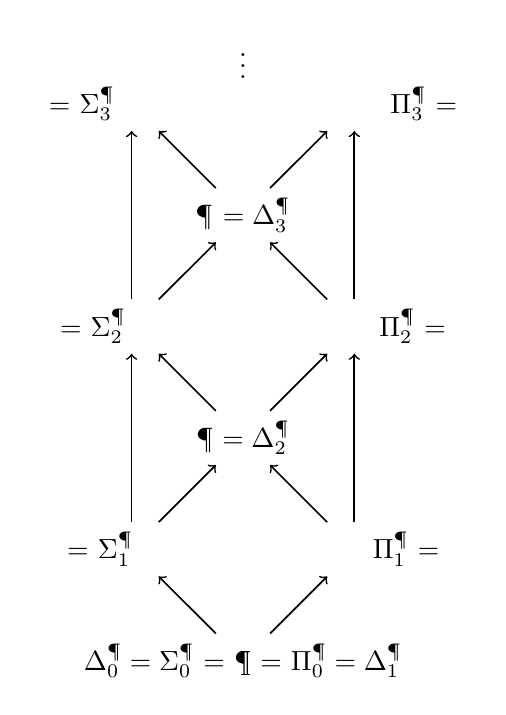
\begin{tikzpicture}[->, node distance=2cm, semithick]
 \node (P) {$\Delta_0^\text{\P} =\Sigma_0^\text{\P}$ = {\P} = $\Pi_0^\text{\P} = \Delta_1^\text{\P}$};
 \node (Sigma1) [above left of=P]       {{\NP} = $\Sigma_1^\text{\P}$ \hspace*{0.8cm}};
 \node (Pi1)    [above right of=P]      {\hspace*{1.2cm} $\Pi_1^\text{\P}$ = \coNP};
 \node (Delta2) [above left of=Pi1]     {$\text{\P}^\text{\NP} = \Delta_2^\text{\P}$ };
 \node (Sigma2) [above left of=Delta2]  {$\text{\NP}^\text{\NP}$ = $\Sigma_2^\text{\P}$ \hspace*{1.0cm}};
 \node (Pi2)    [above right of=Delta2] {\hspace*{1.5cm} $\Pi_2^\text{\P}$ = $\text{\coNP}^\text{\NP}$};
 \node (Delta3) [above left of=Pi2]     {$\text{\P}^{\text{\NP}^\text{\NP}} = \Delta_3^\text{\P}$};
 \node (Sigma3) [above left of=Delta3]  {$\text{\NP}^{\text{\NP}^\text{\NP}}$ = $\Sigma_3^\text{\P}$ \hspace*{1.3cm}};
 \node (Pi3)    [above right of=Delta3] {\hspace*{1.8cm} $\Pi_3^\text{\P}$ = $\text{\coNP}^{\text{\NP}^\text{\NP}}$};
 \node (dots)   [above of=Delta3]       {\vdots};
 \draw (P)      -> (Sigma1);
 \draw (P)      -> (Pi1);
 \draw (Sigma1) -> (Sigma2);
 \draw (Sigma1) -> (Delta2);
 \draw (Pi1)    -> (Pi2);
 \draw (Pi1)    -> (Delta2);
 \draw (Delta2) -> (Sigma2);
 \draw (Delta2) -> (Pi2);
 \draw (Sigma2) -> (Sigma3);
 \draw (Sigma2) -> (Delta3);
 \draw (Pi2)    -> (Pi3);
 \draw (Pi2)    -> (Delta3);
 \draw (Delta3) -> (Sigma3);
 \draw (Delta3) -> (Pi3);
\end{tikzpicture}
\caption{Polynomial Hierarchy, taken from http://commons.wikimedia.org/wiki/File:Polynomial\_time\_hierarchy.svg. Each arrow represents inclusion: for example, $\Sigma_1^\text{\P} \subseteq \Delta_2^\text{\P} \subseteq \Sigma_2^\text{\P}$.}
\end{figure}